\documentclass[12pt, a4paper, french, openright]{report}
% version reliée
% \documentclass[11pt, a4paper, french, openright, twoside]{report}
\usepackage[french]{babel}
\selectlanguage{french}
\usepackage[T1]{fontenc}
\usepackage[utf8]{inputenc}
\usepackage{lmodern,textcomp}
\usepackage[
    left = \flqq,%
    right = \frqq,%
    leftsub = \flqq,%
    rightsub = \frqq%
]{dirtytalk}

\usepackage{csquotes}
\usepackage{hyperref}

\usepackage{graphicx}
\usepackage{caption}
\usepackage{setspace}

\usepackage{titling}

\usepackage[backend=biber]{biblatex}
\bibliography{bibliography}

\newcommand{\HRule}{\rule{\linewidth}{0.5mm}}
\renewcommand{\thefootnote}{\alph{footnote}}

\usepackage{fancyhdr}
\pagestyle{fancy}
\fancyhf{}
\renewcommand{\chaptermark}[1]{\markboth{\bsc{\chaptername~\thechapter{} :} #1}{}}
\renewcommand{\sectionmark}[1]{\markright{\thesection{} \ #1}}
\renewcommand{\headrulewidth}{0pt}
\lhead[\textsl{\leftmark}]{\textsl{\rightmark}}
\rhead[\textsl{\rightmark}]{\textsl{\leftmark}}
\cfoot[\thepage]{\thepage}
\setlength{\headheight}{15pt}

\let\headruleORIG\headrule
\renewcommand{\headrule}{\color{black} \headruleORIG}
\renewcommand{\headrulewidth}{1.0pt}
\usepackage{colortbl}
\arrayrulecolor{black}

\renewcommand{\footrulewidth}{0.4pt}% 

\usepackage{sectsty}
\usepackage{lipsum}% just to generate some text

\chaptertitlefont{\centering \MakeUppercase}




\title{Comment le système de recommandation de Netflix a rendu
accros ses utilisateurs ?}

\author{Fabien MICHEL}

\date{\today}

\begin{document}

\begin{titlepage}
\begin{center}

% Upper part of the page. The '~' is needed because only works if a paragraph has started.

\includegraphics[width=1\textwidth]{./upn}~\\[1cm]

\textsc{\Huge Master 2 MIAGE}\\[0.5cm]

\textsc{\huge Mémoire de fin d'études}\\[1.5cm]



% Title
\HRule

{\huge \bfseries \thetitle \\[0.4cm] }


\HRule

\vspace{5mm}

% Author and supervisor
\begin{minipage}{0.4\textwidth}
\begin{flushleft} \large
\emph{Auteur:}\\
Fabien \textsc{MICHEL}
\end{flushleft}
\end{minipage}
\begin{minipage}{0.4\textwidth}
\begin{flushright} \large
\emph{Tuteurs entreprise :} \\
\emph{Référent:} \\
Lom messan \textsc{HILLAH}
\end{flushright}
\end{minipage}

\vfill

% Bottom of the page
{\huge Promotion 2018-2019}

\end{center}
\end{titlepage}

%page blanche
\newpage
~
%ne pas numéroter cette page
\thispagestyle{empty}
\newpage

%ne pas numéroter cette page
\thispagestyle{empty}
\begin{center}
\subsection*{Remerciements}
\end{center}

\hskip7mm

\begin{spacing}{1.3}
La réalisation de ce mémoire a été possible grâce au concours de plusieurs personnes à qui je voudrais témoigner toute ma gratitude.

\vspace{5mm}

Je tiens à exprimer toute ma reconnaissance à mon tuteur de mémoire, Monsieur Lom messan {HILLAH}. Je le remercie de m’avoir encadré, orienté, aidé et conseillé.

\vspace{5mm}

J’adresse mes sincères remerciements à tous les professeurs, les intervenants et à toutes les personnes qui par leurs paroles, leurs écrits, leurs conseils et leurs critiques ont guidé mes réflexions et qui ont accepté de me rencontrer et de répondre à mes questions durant mes recherches.

\vspace{5mm}

Je tiens tout particulièrement à remercier Marjolaine {LEVEAU} pour ses conseils et ses remarques qui m'ont guidé et m'ont été d'une très grande aide durant la rédaction de ce mémoire.

\end{spacing}


\newpage
%ne pas numéroter cette page
\thispagestyle{empty}
\newpage

%ne pas numéroter cette page
\thispagestyle{empty}
\begin{abstract}
\hskip7mm
\begin{spacing}{1.3}

Le « Dayli mix » de Spotify, les vidéos recommandés sur la page d’accueil YouTube ou encore les suggestions de d’abonnement sur Instagram, ces recommandations sont exclusivement basées sur les J'aime ou interactions précédentes. Tous cela est issu d’un système de recommandation, aujourd’hui très présent dans notre quotidien et dans beaucoup de service que nous utilisons. 

Aujourd’hui une entreprise mise beaucoup sur les systèmes de recommandations : Netflix.  Ce service utilisé par des millions d’utilisateur dans le monde met en avant son système de recommandation dans son plan de communication mais estime aussi qu’il s’agit d’un élément primordial pour garder un ses utilisateurs sur sa plateforme. 

Ce mémoire étudie l'algorithme de recommandation de Netflix sous différents aspects.

\end{spacing}
\end{abstract}

\tableofcontents
\thispagestyle{empty}
\setcounter{page}{0}
%ne pas numéroter le sommaire

\newpage
~
\thispagestyle{empty}
%recommencer la numérotation des pages à "1"
\setcounter{page}{0}
\newpage

\chapter*{Introduction}
\addcontentsline{toc}{chapter}{Introduction}
\markboth{Introduction}{Introduction}
\label{chap:introduction}

L’importance du système de recommandation pour Netflix.

\vspace{5mm}

\begin{figure}[htp]
  \centering
  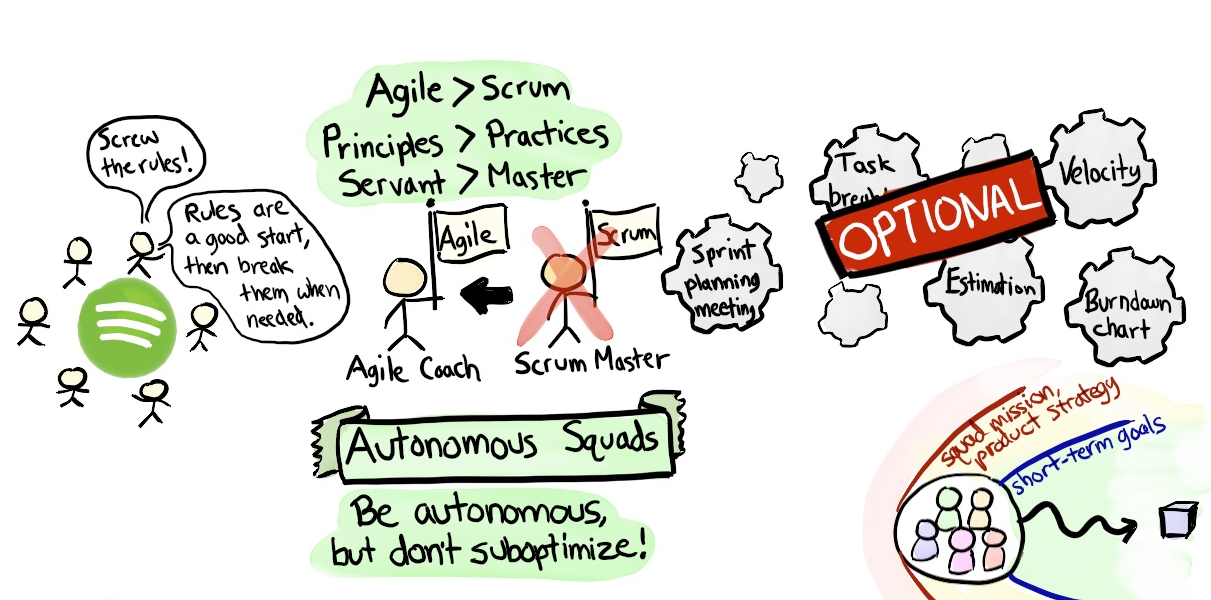
\includegraphics[width=95mm]{./src_img/agile_scrum}
  \caption{Organigramme du LRI.}
  \label{fig:uno}
\end{figure}

\vspace{5mm}

L'entreprise \textbf{Netflix} \supercite{NetflixNumerama} 

\vspace{5mm}



\vspace{5mm}

Les 11 et 12 avril \textit{Reed Hastings} présentait la stratégie de sa société \textbf{Netflix} pour les années à venir à la Cité du Cinéma, renommée \textit{Netflix City} pour l'occasion. Le symbole est fort et à l'image des changements que le service a apporté à l'industrie du divertissement et à notre manière de consommer les films et séries. Tout d'abord créé suite au mécontentement de son créateur à l'égard du service de location de films Blockbuster, alors en position de monopole, il a su se faire une place et créer par la suite un nouveau marché avec son service de vidéo à la demande\footnote{le cheval c'est trop génial}.

\vspace{5mm}
 

\chapter{Contexte et concepts}

%another definition


      
%end of other definition

Aujourd'hui, sur internet des entreprises mettent à disposition de leurs utilisateurs un nombre colossal de données comme YouTube, Amazon ou encore Netflix. Ainsi, il est devenu difficile pour l'utilisateur de trouver des informations pertinentes rapidement. Diverses techniques informatiques se sont développées pour contourner ce problème et ce bien avant les géants d'internet que nous connaissons. Dans le cadre de ce mémoire, nous nous intéresseront essentiellement aux systèmes de recommandation.


\vspace{5mm}

En 1967\supercite{MACQUEEN}, James McQueen applique un algorithme K-moyennes (K-means) permettant de construire des portions de populations homogènes selon plusieurs critères définis à l’avance. Actuellement, cette première étape est considérée comme le début de la recommandation personnalisée. En 1979, est crée Grundy\supercite{Grundy}, il s'agit d'une tentative de recommandation automatique appliquée au métier de bibliothécaire. A l'aide d'une interview, le système classe les utilisateurs en "stéréotypes" permettant ainsi de recommander différents livres en fonctions de leurs "stéréotypes". Nous pouvons considérer qu'il s'agit de la première réelle application d'un système de recommandation. 



\section{Généralités}

Un système de recommandation est une forme spécifique de filtrage de l’information qui a pour but de présenter à un utilisateur des éléments qui sont susceptibles de l’intéresser. Ce système fonctionne en se basant sur les préférences et le comportement d'un utilisateur ou d'un groupe d'utilisateur. In fine, un système de recommandation tente donc de prédire si un élément suggéré est  succeptible d'être apprécié par un utilisateur donné. 

\vspace{5mm} 

Aujourd'hui, les systèmes de recommandations sont devenus êxtremements populaires, ils sont utilisés dans de nombreuses webapp et appliqués à de nombreux domaines comme la publicité, la vente de masse ou encore la consommation de contenu.

\vspace{5mm}

Actuellement, le nombre de données collectées par des entreprises comme Google par exemple, augmente de façon exponentielle, en raison de cette croissance l'importance des systèmes de recommandation augmente tout autant. Depuis les années 90, les systèmes de recommadation sont devenus un domaine de recherche autonome et en recherche constante d'évolution\supercite{ieee}.



%l'intérêt des utilisateurs. Ancien travail [10] distingue recommandation
%techniques en suivant quatre classes.

\section{Les différentes approches}

%[http://citeseerx.ist.psu.edu/viewdoc/download?doi=10.1.1.695.6428&rep=rep1&type=pdf]

%[https://interstices.info/les-systemes-de-recommandation-categorisation/]

Il existe une multitude de type de données avec chacunes des spécificités différentes. Pour être le plus efficace possible, il existe différentes implémentations des systèmes de recommandation afin de traiter au mieux les données utilisateurs permettant d'apporter l'information la plus pertinante possible.

\vspace{5mm} 

En me basant sur les travaux d'Elsa NEGRE\supercite{elsaNegre}(Maître de Conférences à l'Université Paris - Dauphine), j'ai pu déterminer l'existance de 3 grands types de systèmes de recommandation : basé sur un filtrage collaboratif, filtré sur le contenu et enfin les systèmes hybrides. Chacun de ses types de systèmes de recommandation permet de s'adapter au mieux en fonction des différents besoins.


\subsection{Le filtrage collaboratif}

Les systèmes basés sur le filtrage collaboratif construisent des recommandations en observant  la similarité entre les préférences d’un utilisateur et celles d’autres utilisateurs. Ce système ne permet pas d'analyser ou d'étudier les éléments à recommander mais à faire des prévisions basées sur les intérêts d'un utilisateur comparé à un ensemble d'utilisateurs ayant un profil similaire. Dans ce système, on suppose que plus le profil d'un utilisateur est proche d'un ensemble/groupe d'utilisateur alors ils auront tendance à aimer les mêmes éléments. 

\vspace{5mm}

\begin{figure}[htp]
  \centering
  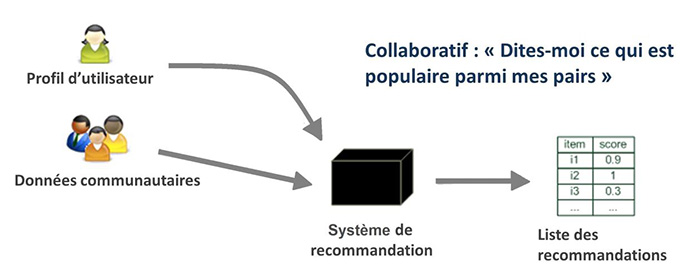
\includegraphics[width=95mm]{./src_img/rs-collaboratif}
  \caption{Un système de recommandation collaboratif\supercite{RSIntro}.}
  \label{fig:duo}
\end{figure}

\vspace{5mm}


Lorsqu'il y a des milliards de produits et un nombre conséquent de clients, il faut une énorme puissance de calcul pour calculer les recommandations. Il existe donc un problème sur l'évolutivité de ce système de recommandation. Lors de la première inscription d'un utilisateur, il est impossible de recommander des produits à cet utilisateur. Ce problème du démarrage a froid est contournable en demandant les préférences d'un utilisateur après son inscription. 

\vspace{5mm}

Aujourd'hui, Amazon a un algorithme de recommandation pour sa boutique. C'est un algorithme utilisant le filtrage collaboratif et plus spécifiquement "Item-To-Item". Lors de la lecture de la fiche "produit d'un article", Amazon suggère une liste d'autres produits en fonctions des clients ayant déjà acheté ce produit. Amazon personnalise aussi sa page d'accueil en fonction des achats précèdents ou des articles dans le panier du client. 

\vspace{5mm} 

\textit{« L’algorithme d’Amazon.com est basé sur le filtrage collaboratif appliqué aux éléments (Item-based collaborative filtering ou Item-to-Item). Le calcul en temps réel de cet algorithme s’adapte à la fois au nombre de clients et au nombre de produits dans le catalogue. L’algorithme construit une matrice de produits similaires en trouvant les produits que les clients ont tendance à acheter ensemble. »}\supercite{elsaNegre}

\vspace{5mm}

\begin{figure}[htp]
  \centering
  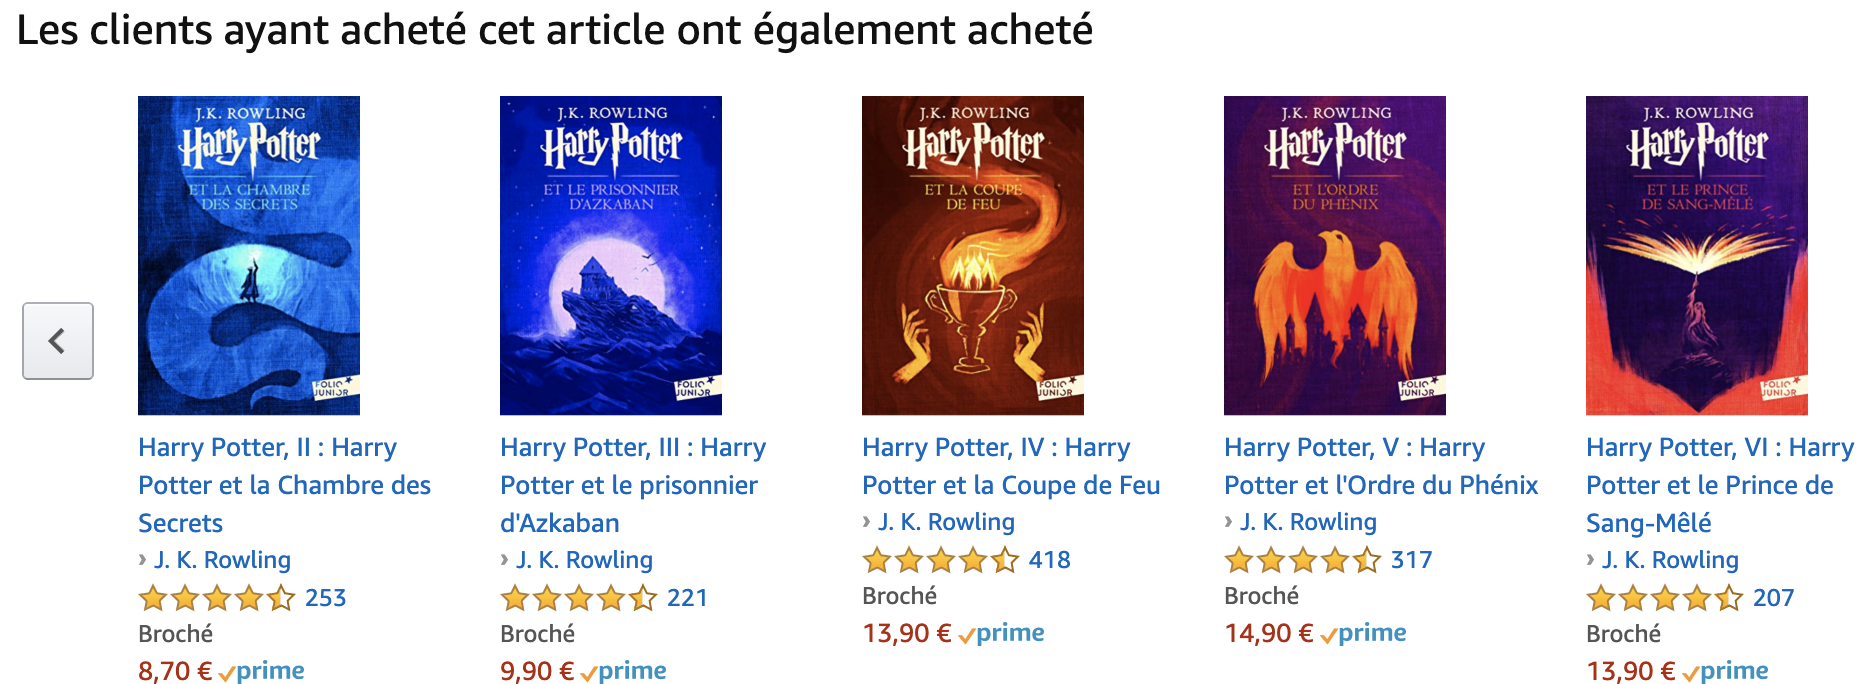
\includegraphics[width=95mm]{./src_img/rs-collaboratif-sample}
  \caption{Amazon et la recommandationn collaborative.}
  \label{fig:duoB}
\end{figure}

\vspace{5mm}




\subsection{Le filtrage basé sur le contenu}

Pour les algorithmes de recommandation basés sur le contenu, le travail consiste à faire concorder les éléments du catalogue qui coïncident le mieux avec les préférences d'un utilisateur. Contrairement au filtrage collaboratif, ce type d'algorithme ne demande pas d'avoir un grand nombre d'utilisateur et peux s'appliquer à des structures plus petites. 

\vspace{5mm}


\begin{figure}[htp]
  \centering
  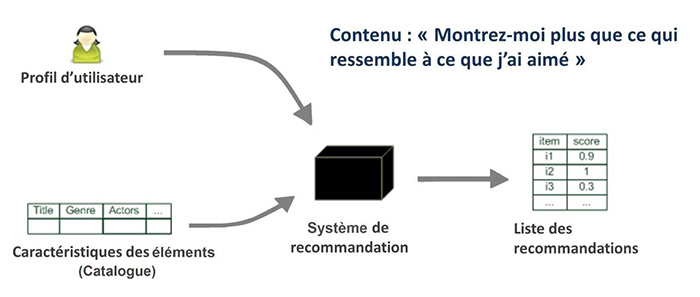
\includegraphics[width=95mm]{./src_img/rs-content}
  \caption{Un système de recommandation basé sur le contenu\supercite{RSIntro}.}
  \label{fig:trio}
\end{figure}

\vspace{5mm}


Premièrement, pour mettre en place ce type de recommandation, chaque éléments ou produits sont décrits par un nombre de caractéristiques connus et finis. Pour chaque utilisateur, il faut expirmer sous forme d'une liste ses intérêts et ses caractériques à nos produits ou nos éléments. 

\vspace{5mm}


La seconde étape pour la mise en place d'un algorithme de recommandation basé sur le contenu est de faire coïncider les caractéristiques des éléments et le profil de l’utilisateur. Ainsi, cela peut être mesuré de différentes manières :

\vspace{5mm}


\begin{itemize}
    \item \textbf{La mesure de similarité.}
    \vspace{2mm}
    \item \textbf{Le TF-IDF} (Term Frequency-Inverse Document Frequency) : consiste à déterminer un score de pertinence.  
    \vspace{2mm}
    \item \textit{«\textbf{Les techniques basées sur la similarité des espaces vectoriels} (les approches bayésiennes, les arbres de décision, etc.) couplées avec des techniques statistiques, lorsqu’il y a trop de mots-clés.»}\supercite{elsaNegre}

\end{itemize}

\vspace{5mm}



Les systèmes de recommandation basés sur le contenu présentent de nombreux avantages dont le démarrage à froid. Si un nouvel élément est ajouté au catalogue, il est simple de le recommander directement aux utilisateurs en fesant correspondre les caractéritiques et les centres d'intérêts d'un utilisateur. Avec ce système de recommandation, une personne avec des goûts atypiques différents de ceux de la base d'utilisateurs habituels n'est pas un problème. Pareil pour les éléments à recommander, un produit peu vendu ou atypique peu coïncider avec les goûts d'un nombre réduit d'utilisateur et donc être recommandé. 

\vspace{5mm} 

Malgrès les nombreux avantages que représente ce système de recommandation, il ne peut pas être appliquable à tous les utilisateurs. Les utilisateurs ayant consulté un grand nombre d’éléments posent un problème (une énorme masse d'information dans le profil de l’utilisateur à faire correspondre avec les propriétés des différents  éléments) et lorsqu’il n’existe pas d’historique (dans le cas d'un utilisateur qui commence à utiliser le système) par conséquence la recommandation pour ces deux cas peut-être difficile. Concernant les éléments à recommander, il est difficile de différencier deux éléments avec des caractéristiques similaires. Une étape difficile est la définition des caractéristiques de chaque utilisateur ainsi que la prise en compte de l'évolution des goûts et par conséquent des caractéritiques des utilisateurs.




\subsection{Le filtrage hybride}

Un système de recommandation hybride combine les approches collaboratives et basées sur le contenu. \textit{«Ce système de recommandation, peut utiliser à la fois  des connaissances extérieures et les caractéristiques des éléments, combinant ainsi des approches collaboratives et basées sur le contenu.»}\supercite{elsaNegre}


\vspace{5mm}

\begin{figure}[htp]
  \centering
  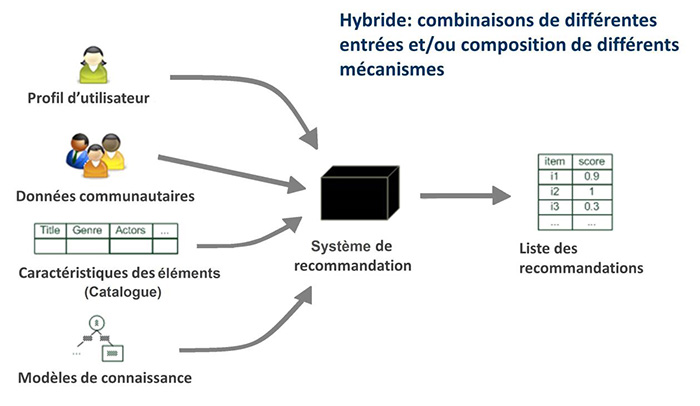
\includegraphics[width=95mm]{./src_img/rs-hybride}
  \caption{Un système de recommandation hybride\supercite{RSIntro}.}
  \label{fig:quatro}
\end{figure}

\vspace{5mm}

L'approche hybride est une combinaison de différentes approches, par conséquent sont but étant de présenter les avantages des approches qui la composent tout en limitant leurs inconvénients respectifs. Actuellement, il existe différentes catégories de combinaisons de systèmes de recommandation pour la création d'un système de recommandation hybride\supercite{RobinBurke,RSIntro}: 

\vspace{5mm}


\begin{itemize}
    \item \textbf{La combinaison monolithique} (monolithic hybridization design)\supercite{elsaNegre} : décrit une conception de l'approche hybride intégrant les aspects de différentes stratégies de recommandation en un seul algorithme.
    \vspace{2mm}
    \item \textbf{La combinaison parallèle} (parallelized hybridization design)\supercite{elsaNegre} : décrit une conception de l'approche hybride où sur la base de données d’entrée commune, les systèmes de recommandation fonctionnent de façon parallèles et indépendantes. Chacun produit une liste de recommandations distincte. Une étape ultérieure d’hybridation est nécessaire permettant de combiner le résultat en un ensemble final de recommandations.
    \vspace{2mm}
    \item \textbf{La combinaison tubulaire} (pipelined hybridization design)\supercite{elsaNegre} : décrit une conception de l'approche hybride où plusieurs systèmes de recommandation sont joints. Les données de sortie d’un système de recommandation devient une partie des données d’entrée du système de recommandation suivant.
    
\end{itemize}

\vspace{5mm}

\section{Le machine learning}

%http://penseeartificielle.fr/difference-intelligence-artificielle-machine-learning-deep-learning/#Le_machine_learning

\textit{«
Les systèmes de recommandation sont couramment utilisés en lien avec l’intelligence artificielle. Leurs capacités à fournir un aperçu global, à prédire les événements et à mettre en évidence des corrélations contribuent à expliquer leurs utilisations en IA. Par ailleurs, les techniques de Machine Learning sont fréquemment utilisées pour créer les algorithmes de recommandation. Par exemple, chez Arcbees, un système de prédiction des préférences de films a été construit, il utilise un réseau de neurones et les données de IMDb. Les réseaux de neurones peuvent effectuer rapidement des tâches complexes et manipuler facilement des données massives. En fournissant une liste de films comme entrées et en comparant la sortie avec la note de l’utilisateur, le réseau peut apprendre par lui-même la règle permettant de prédire les évaluations futures d’un utilisateur spécifique.»}\supercite{MachineLearn}

\section{L'approche de netflix}

%https://www.futura-sciences.com/tech/questions-reponses/informatique-netflix-fonctionne-algorithme-recommandations-8640/

%https://uxplanet.org/netflix-binging-on-the-algorithm-a3a74a6c1f59



Chez Netflix 80\%\supercite{p80} du contenu consommé par les utilisateurs est issu d'une recommandation. Fort de ce constat, le rôle du système de recommandation occupe une place centrale autant pour Netflix que pour ses utilisateurs. Ce système repose sur les utilisateurs, les caractéristiques des contenus et un algorithme. 

\vspace{5mm} 

Pour comprendre le besoins de ses utilisateurs, Netflix fait une analyse comportementale précise de chaque utilisateur. Ainsi, un contenu consommé sera utilisé pour recommander des series ou des films. Dans ce cas, Netflix utilise le machine learning pour dresser le portrait le plus précis possible de chaque utilisateur dont notamment : 


\vspace{5mm}


\begin{itemize}
    \item \textbf{La navigation précise}: combien de temps l'utilisateur met à trouver un contenu  et par quel moyen (strates, catégories,...).
    \vspace{2mm}
    \item \textbf{La temps de lecture d'un contenu }: permettant de déterminer si un contenu lancé est regardé en entier, à moitié ou partiellement  
    \vspace{2mm}
    \item \textbf{La notion de temps} : en fonction de la période de l'année, un type de contenu peut-être plus consommé par exemple les films de noël. Mais aussi en fonction de l'heure, par exemple en début de soirée peut-être que les utilisateurs consomment plus de films que de séries. 
    \vspace{2mm}
    \item \textbf{L'avis donné par l'utlisateur} : L'utilisateur peut donner son avis sur un contenu avec un icone "pouce vers le haut" ou "pouce vers le bas". 
\end{itemize}

\vspace{5mm}
%https://www.wired.co.uk/article/how-do-netflixs-algorithms-work-machine-learning-helps-to-predict-what-viewers-will-like

Une analyse du comportement seule ne permet pas de déterminer les séries et films à recommander à un utilisateur, il faut analyser le contenu et faire concorder le portrait de chaque utilisateur avec le contenu. L'ensemble du catalogue disponible sur Netflix est indexé pour décrire au mieux un centenu selon une immense bibliothèque de mots-clés. Le rôle de l'algorithme de machine learning est d'ordonnancer les données des utilisateurs et les contenus indexés. En pratique, le système de recommandation de Netflix appélé Cinematch analyse les scores cumulés de chaque contenu en utilisant une variante du coefficient de corrélation de Pearson avec tous les autres films afin de déterminer une liste de films « semblables » qui sont susceptibles de plaire à l'utilisateur. Puis, la partie en ligne et en temps réel du système calcule une régression multivariée\footnote{Le modèle de régression linéaire multiple est l’outil statistique le plus habituellement mis en œuvre pour l’étude de données multidimensionnelles. Cas
particulier de modèle linéaire, il constitue la généralisation naturelle de la régression simple.} basée sur ces corrélations pour déterminer une prédiction unique et personnalisée pour chaque film recommandable fondée sur ces scores.

%https://uxplanet.org/netflix-binging-on-the-algorithm-a3a74a6c1f59
%https://www.wired.co.uk/article/how-do-netflixs-algorithms-work-machine-learning-helps-to-predict-what-viewers-will-like
%https://mobilesyrup.com/2017/08/22/80-percent-netflix-shows-discovered-recommendation/

\chapter{Problématique et contraintes}



\section{Généralités}
Afin de fonctionner correctement et d'être efficace pour une population donnée, un algorithme de recommandation fait face à un certain nombre de contraintes selon son type : 


\vspace{5mm}


\begin{itemize}
    \item \textbf{Item cold start} : C'est lorsqu'un item est nouveau ou simplement lorsque l’item n’a pas encore été « cliqué » ou « acheté ». Cet item est difficilement recommandable via des algorithmes de recommandation de type collaborative filtering. En employant des méthodes de type content-based un nouvel item est facilement recommandable même si cet item est nouveau.
    \vspace{2mm}
    \item \textbf{User cold start} : Si un utilisateur est nouveau, il existe aucun historique d’interaction avec le système. Il faut alors avoir recours à des données extérieures pour pouvoir commencer à recommander des items pertinents comme des données extraites des réseaux sociaux ou une demande explicite des goûts des nouveaux utilisateurs.  
    \vspace{2mm}
    \item \textbf{Diversity} : Ce problème survient souvent lors de l’utilisation de méthodes de type "contentbased filtering", le système recommande toujours les mêmes items à un utilisateur, ce qui l’enferme sans possibilité d’exploration en dehors des intérêts détectés par le système.
    \vspace{2mm}
    \item \textbf{Grey sheep} : certains utilisateurs ne font rien comme les autres, on ne peut donc pas leur recommander d’item via les méthodes de type collaborative filtering. 
    \vspace{2mm}
    \item \textbf{Quality} : le content based filtering analyse le contenu, mais la qualité du produit n'est pas forcement déterminé par son contenu (A survey on recommendation system de Singh et al.).
    \vspace{2mm}
    \item \textbf{Trust} : les utilisateurs doivent avoir confiance et croire en la performance du système pour continuer à l’utiliser.
    
\end{itemize}

\vspace{5mm}

Il existe un grand nombre d’autres contraintes comme \textbf{Scalability}, \textbf{Privacy}, et bien d’autres.



\section{Les contraintes et problématiques de Netflix}


A la création d'un compte Netflix, pour contourner le problème de l’\textbf{User Cold Start} le système demande à l'utilisateur de choisir un ensemble de séries ou de films qu'il aime déjà. Ainsi le système de recommandation de Netflix peut commencer à recommander d'autres contenus. Les contenus recommandés doivent être de bonne qualité (contrainte \textbf{Quality}) sinon l’utilisateur lassé n’utilisera plus le service. 

\vspace{5mm}

Chaque mois, Netflix met à disposition de nouveaux programmes originaux sur sa plateforme et donc se retrouve face à la contrainte \textbf{Item-Cold-Start}. Ce contenu étant nouveau, il manque d’avis permettant de déterminer sa qualité. Les programmes sont ainsi mis en avant par la plateforme pour faire leurs promotions mais aussi dans les strates de recommandation en fonction des mots-clés associés. 

\vspace{5mm}

Les abonnements étant mensuels et sans engagement, chaque mois Netflix doit convaincre les utilisateurs de rester sur la plateforme. Ainsi de façon mensuelle, la plateforme subie les contraintes \textbf{Diversity} et \textbf{Trust}. En offrant de nouveaux contenus chaque mois, la plateforme doit convaincre ses utilisateurs que la recommandation est pertinante vis à vis de leurs besoins.

 



\section{L'importance de la recommandation pour Netflix}

%https://medium.com/netflix-techblog/artwork-personalization-c589f074ad76

Avec un catalogue composé de milliers de films et de séries par pays ainsi qu’une base d’utilisateurs grandissante de plusieurs millions d’utilisateurs à travers le monde, il est difficile pour Netflix d’utiliser un unique algorithme pour recommander des contenus.

\vspace{5mm}

Dans un article publié par Netflix\supercite{netflixRS&BusinessValue}, les auteurs (responsables du machine learning chez Netflix) font l'état de six algorithmes présents sur la page d’accueil afin d’afficher une recommandation unique à chaque utilisteur : 

\vspace{5mm}


\begin{itemize}
    \item \textit{« Le \textbf{"Personalized Video Ranker"} opère le classement personnalisé des vidéos et ordonne les 40 rangées de 75 titres qui composent la page d’accueil.}
    
    \vspace{2mm}
    
    \item \textit{Le \textbf{"Top-N Video Ranker"} sélectionne, parmi les contenus les plus populaires dans l’ensemble du catalogue, ceux susceptibles de plaire à l’utilisateur.}
    
    \vspace{2mm}
    
    \item \textit{Le \textbf{"Trending Now"} détermine les tendances à court terme chez les consommateurs : les comédies romantiques de la Saint-Valentin ou les films de Noël, par exemple.}
    
    \vspace{2mm}
    
    \item \textit{Le \textbf{"Continue Watching"} sélectionne les vidéos que l’utilisateur a commencé à regarder et dont il souhaite probablement reprendre la lecture.}
    
    \vspace{2mm}
    
    \item \textit{Le \textbf{"Video-Video Similarity"} choisit les vidéos susceptibles de plaire à un utilisateur, compte tenu des similitudes existantes entre elles et celles qu’il a regardées.}
    
    \vspace{2mm}
    
    \item \textit{Le \textbf{"Page Generation : Row Selection and Ranking"} détermine les rangées à faire figurer sur la page d’accueil et leur ordre d’apparition, en tenant compte des résultats des algorithmes précédents.»}\supercite{franceInfoEnq}
   
\end{itemize}

\vspace{5mm}

%http://www.internetactu.net/2017/10/25/tout-est-recommandation-comment-netflix-sest-transforme/

Selon leurs études, un utilisateur de Netflix doit mettre au maximum 90 secondes à choisir un film, au-delà il perd de l'intérêt pour la plateforme. Pour Netflix, cela correspond entre 10 et 20 films proposés ou recommandés. Dans ce cas, si un utilisateur ne lance pas de film, il quitte le service. Le risque à terme est que l’expérience se renouvelle pour un utilisateur et qu’il ne soit plus satisfait de la proposition du contenu et se désabonne. 

\vspace{5mm}

\begin{figure}[htp]
  \centering
  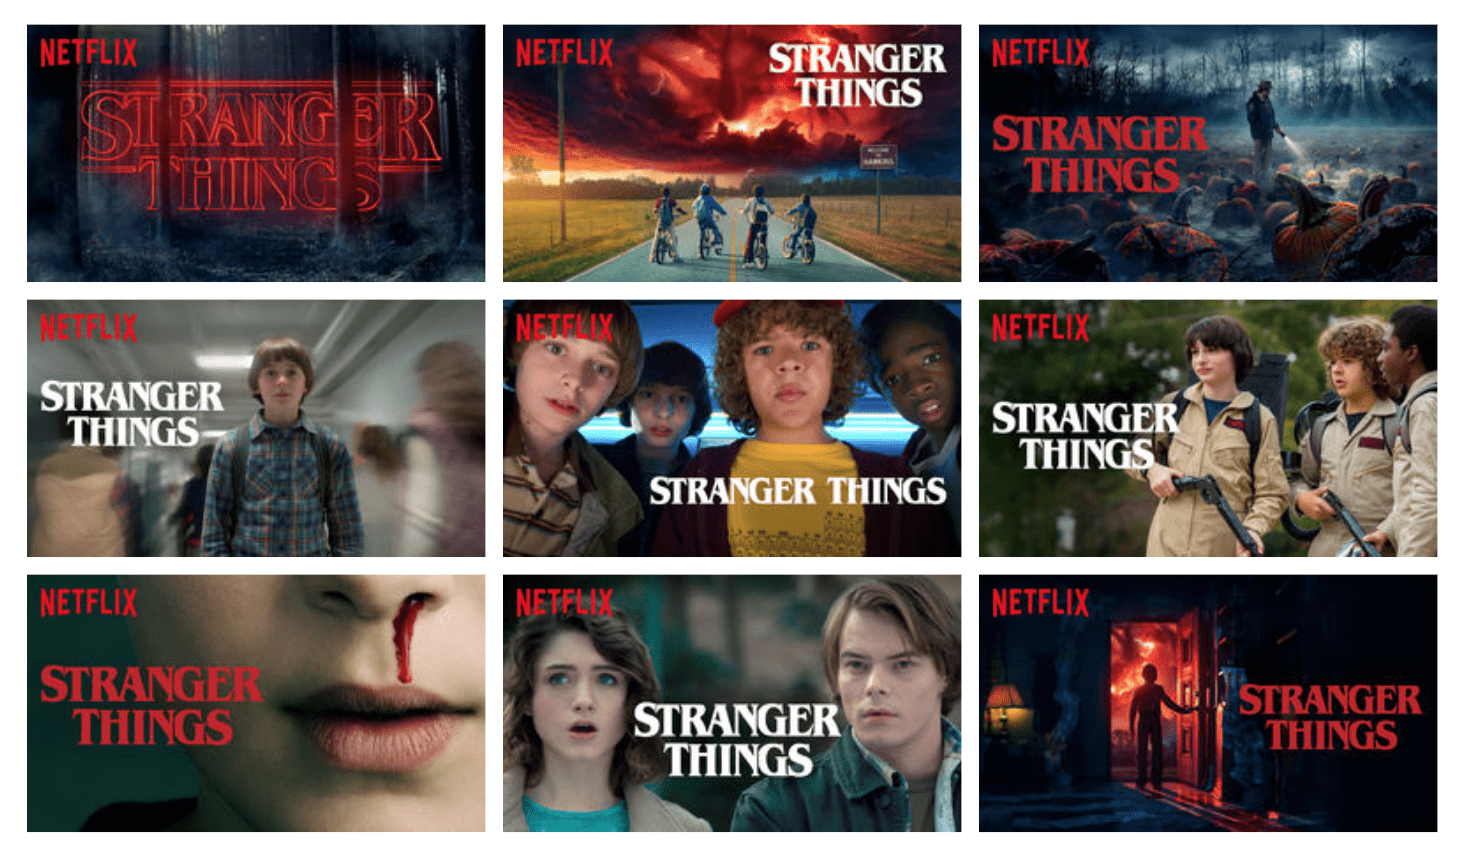
\includegraphics[width=80mm]{./src_img/strangerthings}
  \caption{Exemple de la diversité des illustrations.\supercite{franceInfoEnq}}
  \label{fig:deux-trois}
\end{figure}

\vspace{5mm}

Personnaliser la page d’accueil afin de la rendre unique pour chaque utilisateur est une première étape dans la stratégie de recommandation de Netflix. Lorsqu’un utilisateur navigue dans l’interface, il faut le convaincre de consommer un contenu en moins de 90 secondes.  
Pour rendre sa recommandation plus attractive et personnelle à chaque utilisateur, Netflix a commencé à produire plusieurs illustrations pour chaque contenu. Chaque illustration doit faire ressentir une émotion différente permettant de faire correspondre la vignette du contenu mis en avant avec les goûts de l’abonné.


\vspace{5mm}

\begin{figure}[htp]
  \centering
  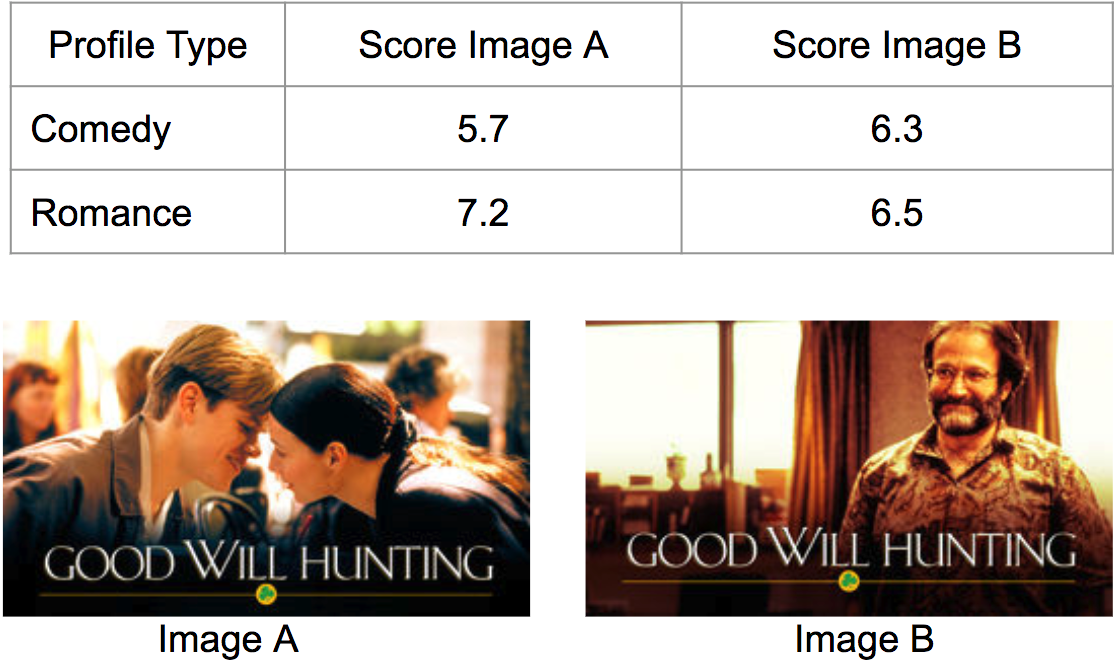
\includegraphics[width=95mm]{./src_img/score}
  \caption{Exemple de score et profil pour le film "Good Will Hunting" .}
  \label{fig:deux-quatre}
\end{figure}

\vspace{5mm}

Si nous prenons l’exemple du film, Good Will Hunting qui est une comédie romantique. 
Un profil qui est déterminé comme regardant principalement des comédies, l’algorithme va choisir la vignette du film mettant en avant Robin Williams un acteur célèbre pour des comédies comme Madame Doubfire par exemple. A l’inverse, si un abonné est déterminé comme préfèrant les contenus romantiques, c’est alors l'image d'un couple s'embrassant qui est choisie. Pour chaque vignette, un ensemble de méthode détermine la correspondance sur 10 de chaque illustration avec chaque type (comédie, romance, horreur, science fiction,...). L'algorithme choisit pour chaque profil d'utilisateur, l'illustration qui correspond le mieux à ses goûts. Cette étape est déterminée par le type qui correspond à l'utilisateur et le score de l'illustration le plus élevé pour ce type de profil.  

\vspace{5mm}

En plus de cibler ses abonnés et grâce à ses multiples vignettes pour une seule série, Netflix peut tester la vignette la plus efficace. Permettant ainsi de proposer les vignettes les plus efficaces pour un nouvel abonné mais aussi d’agrandir la fanbase d’une série. Un fan sur cinq\supercite{1/5} de Stranger Things n’avait jamais regardé de contenus horrifiques sur Netflix. 

\vspace{5mm}

Début 2019, Netflix à dévoilé ses résultats trimestriels. Dans ce communiqué\supercite{fornite}, Netflix affirme que ses principaux rivaux sont désormais Fortnite et YouTube. L’entreprise explique que sa présence globale sur les écrans est supérieure à HBO (chaîne qui possède Game of Thrones) mais inférieure à celle de Fornite le phénomène incontesté du jeux vidéo en 2018. Le temps utilisé pour jouer à Fornite n’est pas utilisé pour regarder des séries, des films ou des documentaires sur Netflix. On parle ici d’une bataille de l’attention et finalement d’argent. En effet : l’argent dépensé pour acheter des tenues dans Fornite n’est pas de l’argent investi dans un abonnement mensuel pour Netflix. Ainsi, plus que jamais, Netflix doit s'appuyer sur son contenu et sur l’ensemble de son système de recommendation pour convaincre ses utilisateurs de consommer sur leur site et donc de passer du temps sur leur plateforme plutôt que de jouer à Fornite pour gagner la bataille de l'attention. 


%https://medium.com/netflix-techblog/artwork-personalization-c589f074ad76


%https://www.sciencesetavenir.fr/high-tech/data/comment-l-algorithme-de-netflix-vous-rend-accro_115965

%https://usbeketrica.com/article/netflix-personnalisation-illustrations-algorithme


\chapter{État de l’art}
%https://www.thrillist.com/entertainment/nation/the-netflix-prize


En 2006, la recherche sur les algorithmes de recommandation a suscité beaucoup d’intérêt lorsque Netflix a lancé une compétion le \textbf{« Netflix Prize »} pour améliorer son approche et sa recommandation de films.

\vspace{5mm} 

 A cette époque, l’entreprise est encore un service de location de DVD en ligne mais chaque utilisateur pouvait laisser son avis et attribuer une note entre un et cinq au film. Avant le lancement de cette compétition, Netflix avait déjà son système de recommandation \textbf{« CineMatch »}, permettant de suggérer aux clients un certain nombre de films qu’ils seraient susceptibles d’aimer.
L’intérêt était double pour Netflix, une bonne recommandation fidélise son audience et une récompense d’un million de dollars permet de faire un joli coup de pub au service permettant d’augmenter par la suite son chiffre d’affaires. 

\vspace{5mm} 

L’objectif du concours était de construire un algorithme de recommandation qui pourrait surpasser CineMatch de 10 pourcent. Le concours a suscité beaucoup d’intérêt, tant dans le milieu de la recherche que dans celui des amateurs de films surement grâce à la somme mise en jeu. 

\vspace{5mm} 



\section{Analyse de l'existant }

Le Netflix Prize était une compétition ouverte au public avec la possibilité de participer en équipe ou de façon individuelle. Il n’était pas possible de soumettre son résultat plus d’une fois par jours. Les gagnants du concours ont eu l’obligation de publier leurs résultats ainsi que le code et les licences sur Netflix. Permettant ainsi à Netflix d'exploiter le code de l'équipe gagnante. 


\vspace{5mm} 

Pour la compétition, Netflix a mis à disposition un ensemble de données pour les participants à la compétition. L’ensemble des données contient au total : 

\begin{itemize}
    \item \textbf{480,189 Utilisateurs} : Ce sont des abonnés réels mais ils sont anonymisés.
    \vspace{2mm}
    \item \textbf{17 770 films}.
    \vspace{2mm}
    \item \textbf{Des évaluations de films} allant de 1 à 5.
    \vspace{2mm}
\end{itemize}
\vspace{5mm} 
Le répertoire "training set" contenant 17770 fichiers soit un par film. La première ligne de chaque fichier contient l’identifiant du film ensuite chaque ligne suivante du fichier correspond à une note donnée par un client. Le format de donnée est le suivant : 

\begin{verbatim}
Film X:
Identifiant client, évaluation, date
Identifiant client, évaluation, date
...
\end{verbatim}


Le fichier "qualifying.txt", contient les donneés éligibles pour la compétition. Cet immense fichier est composé d’un identifiant de film et un ensemble de couple <IdentifiantClient, Date> associé au film. L’algorithme rendu doit prévoir toutes les évaluations des clients donnés sur les films dans le jeu de données de qualification en se basant sur les informations disponibles sur chaque utilisateur dans les données "trainning set". Le format des données est le suivant : 
\begin{verbatim}

Identifiant Film 3 :
Identifiant Client 5, date11
Identifiant Client 12, date12


Identifiant Film 4:
Identifiant Client 45, date 11
Identifiant Client 54, date 12
\end{verbatim}

Concernant le format du rendu, il faut remplacer <IdentifiantClient, Date> par la prédiction de note pour le film. Par exemple, si les données du fichier "qualify" sont les suivantes :
\vspace{5mm}

\begin{verbatim}
111:
3245,2005-12-19
5666,2005-12-23
6789,2005-03-14
225:
1234,2005-05-26
3456,2005-11-07
\end{verbatim}
Alors le fichier contenant les prédictions doit ressembler au résultat suivant :
\begin{verbatim}
111:
3.0
3.4
4.0
225:
1,0
2.0
\end{verbatim}
Le résultat 3.0 signifie que le client 3245 évalue le film 111 le 19 décembre 2005 avec la note de 3,0 étoiles.




\vspace{5mm} 

Le dernier fichier donné par Netflix pour réaliser cette compétition est le "probe.txt". Sa structure est la même que le fichier permettant de se qualifier à l'exception qu'il ne contient aucune date (simplement des identifiants de film et de client). Les données contenues dans ce fichier font aussi références aux données dans le répertoire "training set". 

\begin{verbatim}

Identifiant Film 3 :
Identifiant Client 5
Identifiant Client 12


Identifiant Film 4:
Identifiant Client 45
Identifiant Client 54
\end{verbatim}


Netflix fournit aussi un morceau de code permettant de calculer le RMSE\footnote{Le Root Mean Square Error est l'écart type des résidus (erreurs de prédiction).} des prévisions calculées et surtout de comparer cette valeur à celui de Cinematch sur les mêmes données. Pour information, le RMSE de Cinematch est de 0,9514 pour les données fournies. 

%http://www.netflixprize.com/faq#probe pour cette valeur.

\vspace{5mm} 


\section{Comparaison des différentes approches}

Au cours de la compétition, beaucoup d'équipes sont parties sur des approches différentes. 
Trois années après le lancement du « Netflix Prize », le challenge est réussi et remporté par l’équipe "BellKor’s Pragmatic Chaos". Leur solution est un aggrégat de plusieurs algorithmes et de différents modèles mais aussi d'équipes ( BellKor\supercite{BellKor},The Pragmatic Theory\supercite{Pragmatic} et The BigChaos\supercite{BigChaos}). Cette solution fut la première à avoir un meilleur RMSE que cinematch et par consequent à donc remporté la compétition. 


\vspace{5mm}

Durant la compétition, certains algorithmes étaient plus populaires que d'autres et sont  apparus régulièrement. Parmi eux, l’algorithme du plus proche voisin et la factorisation matricielle se sont montrés particulièrement efficace\supercite{LessonsFromNetflixPrize}.

\vspace{5mm}

Une approche via l’algorithme du plus proche voisin (Nearest neighbors) permet de déterminer si deux utilisateurs ont des préférences identiques, proches ou éloignés. Dans le cas du Netflix Prize, les notes attribuées aux différents films permettent de calculer le degré de préférence. Des préférences éloignées ne permettent pas de déterminer les goûts ou notes d’un autre utilisateur. Au contraire des préférences identiques indiquent une relation forte entre deux utilisateurs permettant ainsi de déterminer plus facilement les films à recommander et prédire leur note. Une relation modérée obtenue avec des préférence similaires permet aussi de calculer la note d’un film en fonction d’un delta plus ou moins précis. 

\vspace{5mm}

\begin{figure}[htp]
  \centering
  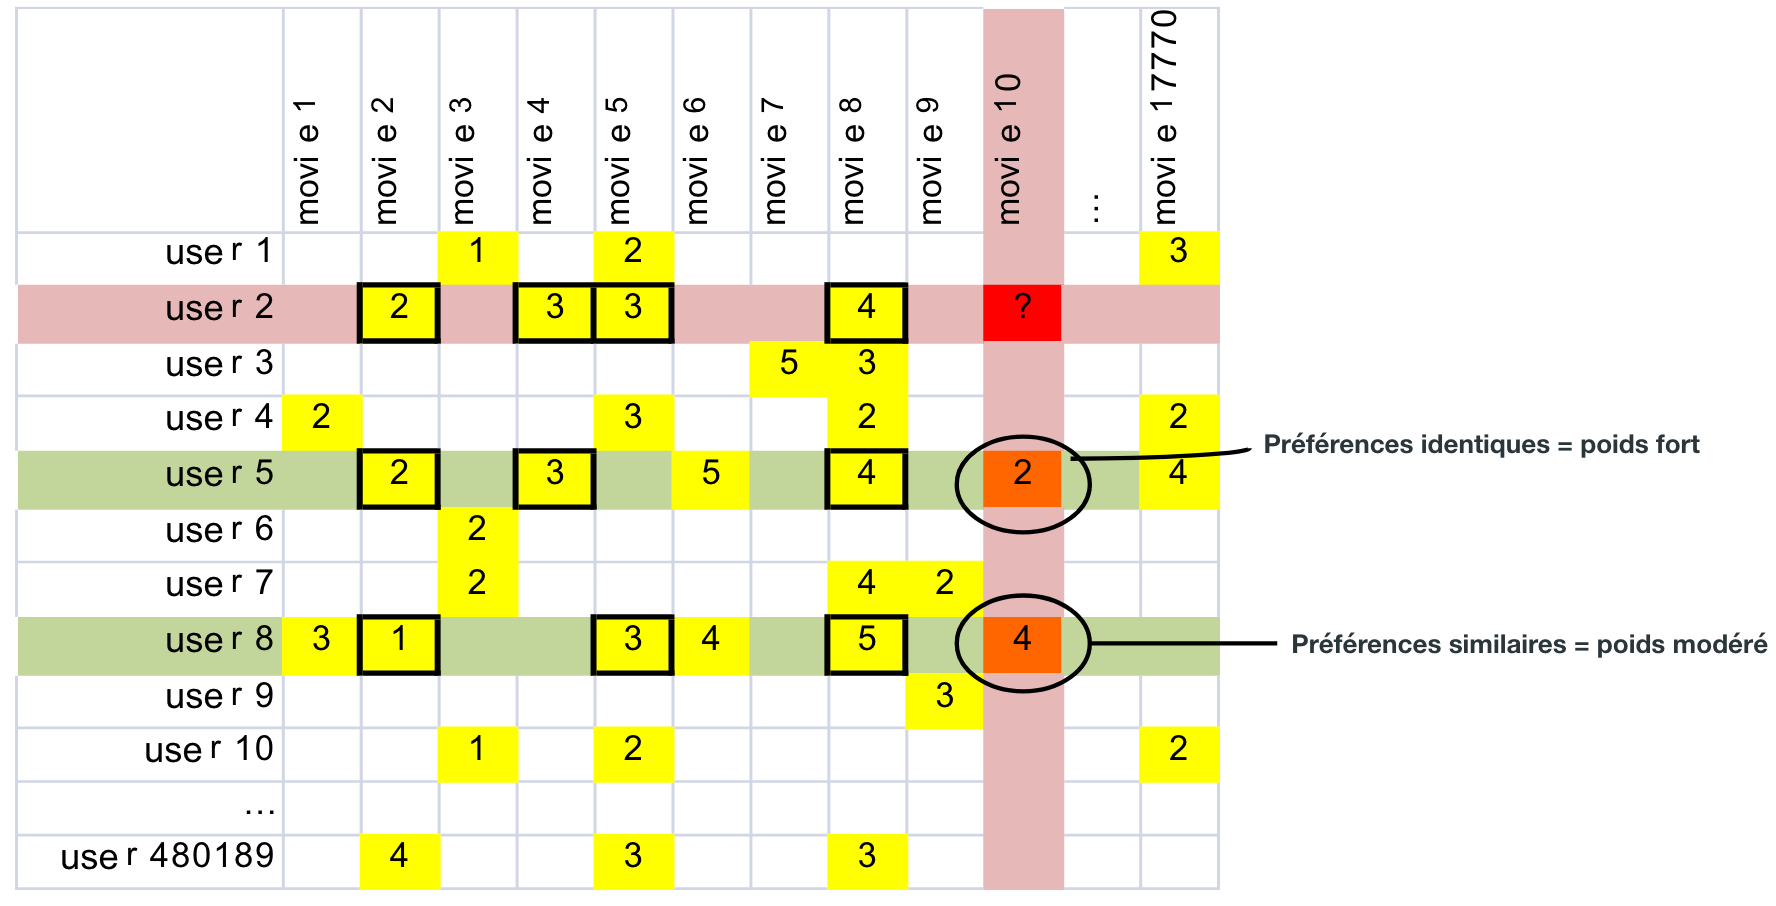
\includegraphics[width=95mm]{./src_img/procheVoisin}
  \caption{Exemple algorithme du plus proche voisin.}
  \label{fig:trois-deux}
\end{figure}

\vspace{5mm}

La factorisation matricielle (Matrix factorization) fait partie des algorithmes de filtrage collaboratif utilisé dans les systèmes de recommandation. Cette approche a prouvé son efficacité au cours du Netflix Prize. Les algorithmes de factorisation matricielle fonctionnent en décomposant la matrice d'interaction "utilisateur-élément" en un produit de deux matrices rectangulaires de plus faibles dimensions. Pour déterminer la note d'un film, il faut alors multiplier et additionner les valeurs pour obtenir la prédiction.

\vspace{5mm}

\begin{figure}[htp]
  \centering
  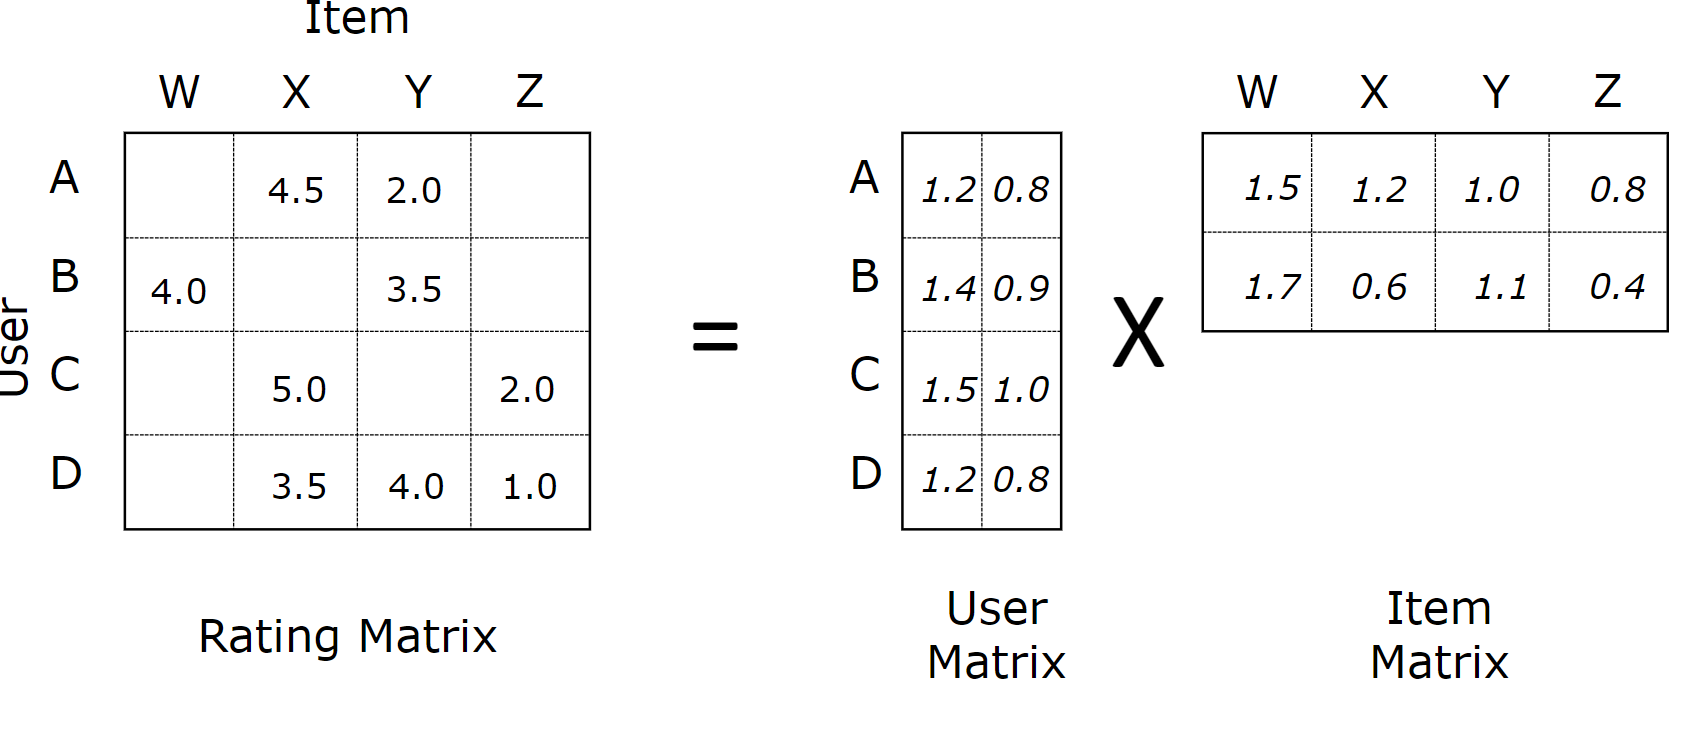
\includegraphics[width=95mm]{./src_img/matrix}
  \caption{Exemple de factorisation matricielle.}
  \label{fig:trois-trois}
\end{figure}

\vspace{5mm}

Ainsi dans l'exemple ci-dessus, la prédiction de l'utisateur A avec l'item W est calculée de la manière suivante : 
\begin{verbatim}

1,2 x 1,5 + 0,8 x 1,7 = 3,16 

\end{verbatim}


L'approche proposée par l’équipe gagnante est articulée autour de 3 axes. Le premier axe modélise les données selon différents niveaux (global, régional et locale). C’est la combinaison de l’extraction des schémas locaux qui sont ensuite factorisés au niveau régional puis affectent globalement les données. Le second axe, est la qualité du modèle, c’est un axe essentiel pour la robustesse permettant la dérivation et les itérations mais aussi d'éviter les effets de débordements lors des factorisations et de l'application d’algorithmes locaux. Afin d’être considérer comme une donnée de qualité et ainsi respecter les critères énoncés il faut que la donnée soit la plus simple possible. Le dernier axe, est une représentation binaire des données selon si les utilisateurs ont donné leur avis de façon implicite ou explicite. Les données sont caractérisées en fonction de leurs évaluations et de la manière dont elles ont été évaluées. Le comportement d’un utilisateur est considéré comme implicite s’il est facile à collecter par son historique de navigation, son historique de location, ses recherches etc... Le retour implicite permet de prédire les évaluations pour les utilisateurs qui n’ont pas encore évalué un film. Quant au retour explicite de l'utilisateur, c'est lorsque ce dernier donne son avis sur le film ou la série par un système de notation (notation du film par une quantité d'étoiles ou bien un symbole de pouce vers le haut ou bien vers le bas). 

\vspace{5mm}

\begin{figure}[htp]
  \centering
  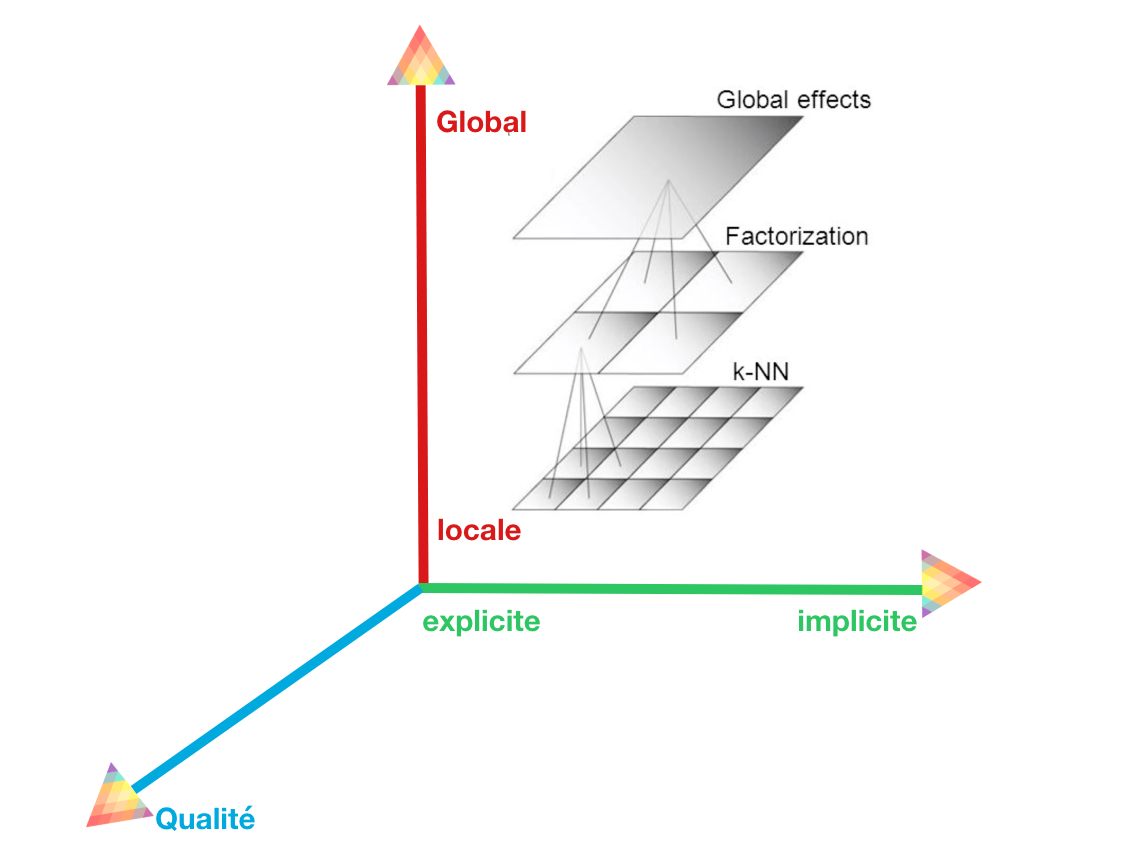
\includegraphics[width=95mm]{./src_img/BPC}
  \caption{Représentation simplifié de la solution BellKor’s Pragmatic Chaos .}
  \label{fig:trois-quatre}
\end{figure}

\vspace{5mm}

%Les solutions proposées sont discutées dans plusieurs articles, notamment [Koren, 2009], [Piotte and Chabbert, 2009] et [Töscher et al., 2009]. Cependant, 

%Malgrès tout le « Netflix Prize » à permis Ce challenge a permis en revanche de mettre en évidence l’intérêt des méthodes de factorisation pour la résolution de problèmes de recommandation, notamment grâce à l’idée d’introduire des informations complémentaires telles que des évaluations implicites, des effets temporels et des niveaux de confiance [Bell and Koren, 2007].
%[Koren, 2009] Koren, Y. (2009). The bellkor solution to the netflix grand prize. Netflix prize documentation, 81.

%[Piotte and Chabbert, 2009] Piotte, M. and Chabbert, M. (2009). The pragmatic theory solution to the netflix grand prize. Netflix prize documentation.

%[Töscher et al., 2009] Töscher, A., Jahrer, M., and Bell, R. M. (2009). The bigchaos solution to the netflix grand prize. Netflix prize documentation, pages 1–52.

%[Bell and Koren, 2007] Bell, R. M. and Koren, Y. (2007). Lessons from the netflix prize challenge. ACM SIGKDD Explorations Newsletter, 9(2) :75–79.

\section{Critique}


Les données mises à disposition pour le Netflix Prize sont issues de réels utilisateurs de Netflix et anonymisées pour des soucis de vie privé. Cependant en 2007, deux chercheurs de l’Université du Texas\supercite{Anonymity} ont réussi à identifier des utilisateurs de façon individuelle par correspondance avec les ensembles de données issues de IMDb\footnote{L’Internet Movie Database (littéralement « Base de données cinématographiques d'Internet »), abrégé en IMDb, est une base de données en ligne sur le cinéma mondial, sur la télévision, et plus secondairement les jeux vidéos.}. 

\vspace{5mm} 

Après une simple étude des données fournies pour réaliser le Netflix Prize, plusieurs choses apparaissent immédiatement comme évidentes. Premièrement, l’ensemble des données fournies est immense avec des variations de notes extrêmes entre les différents utilisateurs. Les variations de note ne permettent pas de déterminer un groupe d’utilisateur semblable facilement. Et deuxièmement, le fichier permettant de s’entrainer et de se qualifier a des propriétés différentes ce qui rajoute une complexité supplémentaire. 

\vspace{5mm} 

Concernant l'utilisation du code de l'équipe gagnante du Netflix Prize,  Xavier Amatriain et Justin Basilico travaillant sur la Science de personnalisation chez Netflix déclarent\supercite{ResultPrize} dans Medium\footnote{Medium est une plateforme web de blog créée en août 2012 par Evan Williams et Biz Stone, les fondateurs de Twitter et Blogger. } : 

\vspace{5mm} 

«A year into the competition, the Korbell team won the first Progress Prize with an 8.43\% improvement. They reported more than 2000 hours of work in order to come up with the final combination of 107 algorithms that gave them this prize. And, they gave us the source code. We looked at the two underlying algorithms with the best performance in the ensemble: Matrix Factorization (which the community generally called SVD, Singular Value Decomposition) and Restricted Boltzmann Machines (RBM). SVD by itself provided a 0.8914 RMSE, while RBM alone provided a competitive but slightly worse 0.8990 RMSE. A linear blend of these two reduced the error to 0.88. To put these algorithms to use, we had to work to overcome some limitations, for instance that they were built to handle 100 million ratings, instead of the more than 5 billion that we have, and that they were not built to adapt as members added more ratings. But once we overcame those challenges, we put the two algorithms into production, where they are still used as part of our recommendation engine.».

\vspace{5mm}

Finalement, même si l'équipe «BellKor's Pragmatic Chaos» a remporté la compétition par un mélange de différents modèles, l'agrégat de plusieurs modèles s'est avéré beaucoup trop coûteux en temps et en énergie pour être mis en place. Dans le reste de l'article, les ingénieures ont mis en avant qu'entre 2006 (date du début de la compétition) et 2009 (fin du concours) les problématiques de Netflix ont changé. Il se pose donc la question de la pertinence d'avoir laissé perdurer cette compétition aussi longtemps. Cependant, selon la citation, les ingénieurs ont déterminé des sous-algorithmes pertinents au sein du travail de l'équipe gagnante. Ce qui a permis d'améliorer les algorithmes de Netflix existants et qui actuellement sont toujours utilisés. 


\chapter{Mon apport}

L'équipe qui à remporté le « Netflix Prize » regroupe plusieurs dizaines de personnes au sein de différentes équipes initiales accumulant plusieurs centaines d’heures de travail et de recherche. Il est évident, que seul et ayant des connaissances limitées des algorithmes et des systèmes de recommandation sur le plan technique, je ne peux rivaliser avec Cinematch ou encore l’équipe gagnante du  « Netflix Prize » . 

\vspace{5mm}

En étudiant la structure de données fournie par Netflix, je me suis posé la question de l’application à une plus grande échelle. Devant le nombre grandissant des plateformes permettant de regarder du contenu mais aussi le suivi sur une chaine de télévision ou via des téléchargements illégaux. Je pense qu’il est possible de générer un algorithme de recommadation pour une plateforme généraliste permettant ainsi de suivre des séries et des films et d'en décrouvrir des nouveaux. 

\vspace{5mm}

Ainsi, lors de l’analyse des données, je me suis rapidement aperçu qu'un manque d’informations sur les films était présent comme notamment le genre associé (Dramatique, Romantique, Comédie, …). Cette information est pourtant essentielle et permet de déterminer avec plus de précision si un utilisateur à une plus forte appétence pour un genre. Je pense que cette information est primordiale lors de la recherche du plus proche voisin, permettant ainsi de rajouter une étape tout en confirmant ou non si la relation entre deux voisins est proche ou extrêmement proche. Il en découle ainsi une augmentation de la précision lors de l'estimation d'un avis, d'une note ou simplement d'une recommandation. 

\vspace{5mm}

Ainsi, pour démontrer la pertinence de mon raisonnement je me suis basé uniquement sur deux types de données. Premièrement, un fichier contenant la liste des 25 plus gros succès du box-office Nord-américain, structuré de la façon suivante : 



\vspace{5mm}

\begin{verbatim}
...
Movie2,1977,Star Wars episode IV : Un nouvel espoir,Science-Fiction
...
\end{verbatim}

\vspace{5mm}

Ici, la donnée importante n’est pas le film en lui-même mais le genre principal associé. Par exemple, "Avatar" est un film de Science-Fiction alors que "Titanic" est un film de Romance. Secondement, il me fallait une structure de données pour les utilisateurs du système. Afin de me simplifier la tâche, un utilisateur est représenté comme une liste de note. Les notes sont comprises de 0 et 5, je considère donc que chaque film vu est obligatoirement noté entre 1 et 5 (1 étant un film non apprécié et 5 un film coup de cœur). Évidemment, un film ayant une note égale à 0 est considéré comme un film non regardé et par conséquent potentiellement recommandable. 

\vspace{5mm}

Au cours du développement de ma solution, initialement j'ai décidé de créer une liste d’utilisateur aléatoirement. Cependant, une génération aléatoire ne permet pas à chaque fois de tomber sur un cas suffisamment pertinent pour démontrer l’efficacité de ma solution dans certains cas précis. Ainsi, j’ai donc décidé de m’orienter vers une liste d’utilisateur défini et d’appliquer mon système de recommandation sur un unique utilisateur permettant de reproduire le cas concret d’un utilisateur qui se connecte sur Netflix. Connaissant les données, je connais aussi le résultat à atteindre vérifiant ainsi la véracité du système. Ci-dessous un schéma des données utilisateurs utilisé :  

\vspace{5mm}


\begin{figure}[htp]
  \centering
  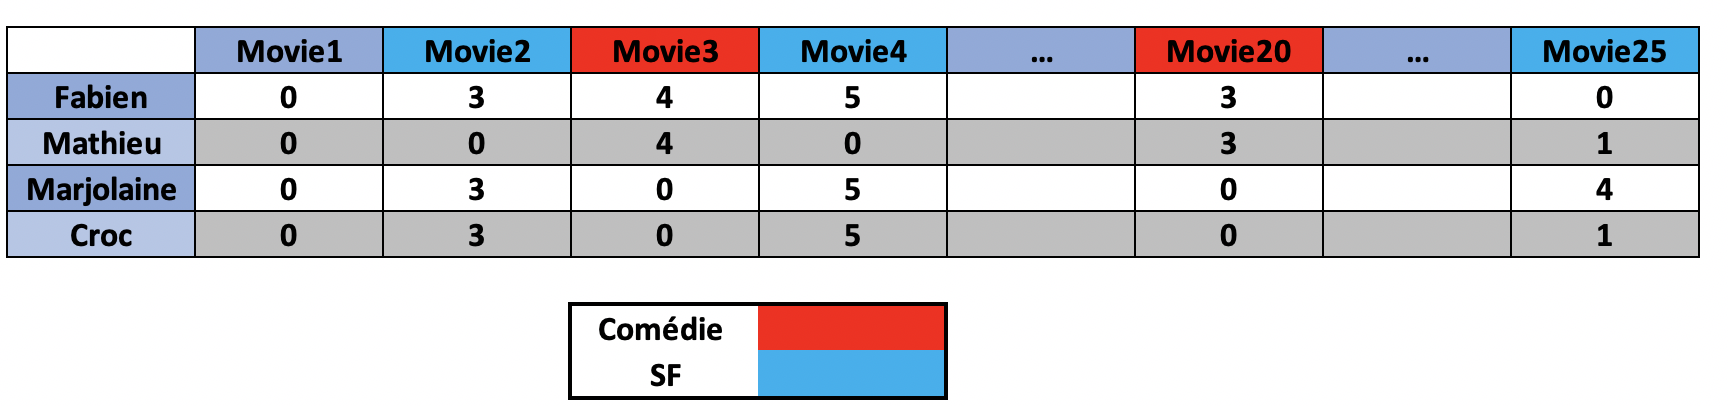
\includegraphics[width=95mm]{./src_img/apport_data}
  \caption{Schéma des données utilisateurs utilisé.}
  \label{fig:a-un}
\end{figure}

\vspace{5mm}

Hormis le profil de « Fabien », nous avons 3 profils utilisateurs. L’utilisateur « Mathieu » est très client des comédies, il a consommé deux films de types Comédie et un film de Science-Fiction le film « movie25 » qu’il n’a malheureusement pas apprécié.  Les profils « Marjolaine » et « Croc » sont friands des films de Science-Fiction, seul leurs notes attribuées au film « movie25 » diffères. 

\vspace{5mm}

Hormis son manque de notation pour « movie25 », le profil  « Fabien » est similaire aux autres profils consommant ainsi des films de Science-fiction et de Comédie. Mon système de recommandation crée en Python aura pour but de prédire la note que Fabien attribuera au film numéro 25 correspondant à "Jurassic World". 


\section{Recherche des plus proches voisins}

Rechercher les plus proches voisins est une méthode très efficace pour créer un groupe d’utilisateur avec des consommations identiques permettant ainsi une recommandation rapide pour un utilisateur donné. Pour rappel, cette méthode a démontré son efficacité lors du Netflix Prize. 

\vspace{5mm}

Concrètement, je prends le  « profil Fabien » et je calcule la distance euclidienne entre les notes attribuées par Fabien et les autres utilisateurs. Mon algorithme des plus proches voisins à une condition supplémentaire, la distance entre Fabien et un autre utilisateur est calculée pour chaque film individuellement et seulement si les deux personnes ont regardé le film sélectionné. La valeur cumulée de la distance euclidienne pour chaque film permet d’obtenir une distance entre Fabien et les autres utilisateurs.  A la fin de cette étape, j’ai une liste de profil organisée de la façon suivante : 

\begin{verbatim}
Distance : données de l’utilisateur Mathieu 
\end{verbatim}

Ensuite, je trie cette liste pour obtenir une liste ordonnée de façon croissante sur la distance. Mais avec ce jeu de données réfléchi, la distance entre Fabien et les autres profils est identique avec une valeur égale à 0, ce qui implique des profils similaires. Au préalable, j’ai défini une limite d’acceptation, dans le cadre de ce mémoire, j’ai choisi de garder les 3 profils les plus proches de l’utilisateur Fabien. 

\vspace{5mm}
 
Ainsi, à la fin de cette étape, les profils :  « Marjolaine, Croc et Mathieu »  sont considérés comme des voisins proches sur lequel une recommandation est possible pour Fabien. 

\begin{figure}[htp]
  \centering
  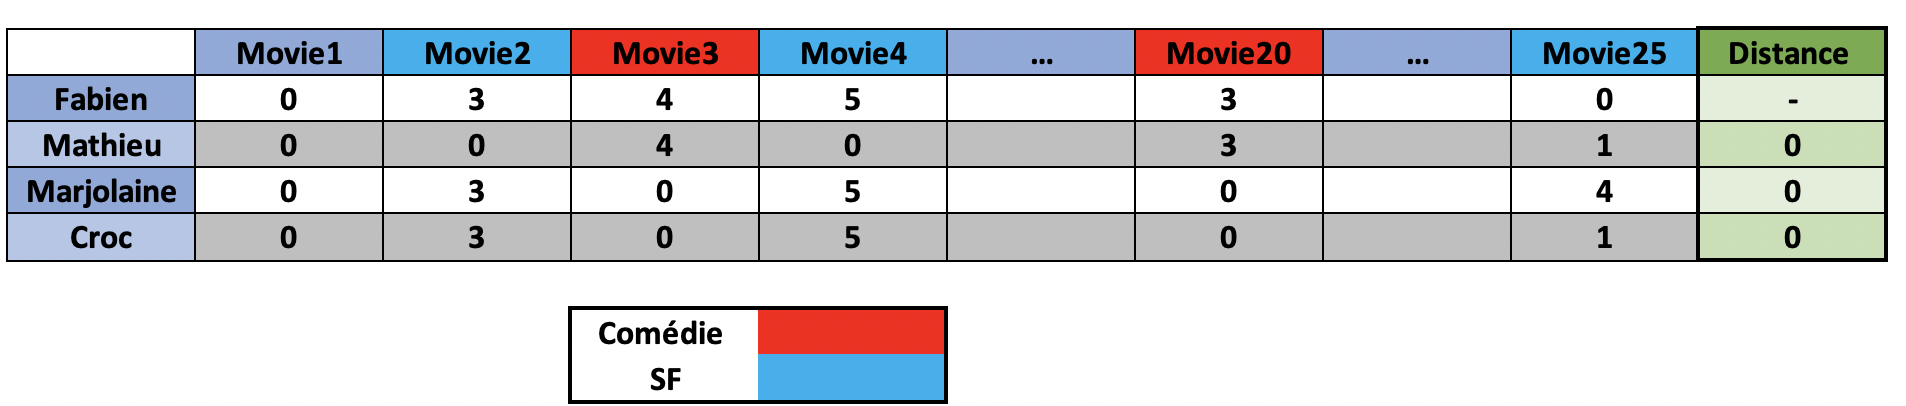
\includegraphics[width=95mm]{./src_img/apport_distance}
  \caption{Recherche des plus proches voisins.}
  \label{fig:a-deux}
\end{figure}

\vspace{5mm}


\section{Trier les voisins selon le film}

En partant des données pour Fabien et sa liste des plus proches voisins, mon système de recommandation va essayer de recommander un ou plusieurs films pour Fabien. Techniquement, pour chaque film non regardé par Fabien, je vais rechercher si parmis ses voisins les plus proches au moins un voisin a regardé ce film. Dans ce cas précis, seul le film "Jurassic World" (« Movie25 ») est éligible.

\vspace{5mm}

Premièrement, je vais enlever de la liste des voisins les plus proches ceux qui n’ont pas regardé ce film. Dans notre cas très précis, aucun voisin n’est évincé. Deuxièmement, je vais appliquer une variante de l’algorithme des plus proches voisins mais basé sur le type du film. Concrètement, "Jurassic World" est un film de Science-Fiction et je vais calculer la note moyenne attribué par Fabien sur les films de type Science-Fiction. Cette moyenne est aussi calculée pour chaque voisin proche restant. 

\vspace{5mm}

Finalement, il faut classer les voisins restant selon leur moyenne attribuée aux films de Science-fiction et non pas par ordre croissant mais selon si leur moyenne est proche ou non de celle de Fabien. Donnant le résultat suivant : 

\vspace{5mm}


\begin{figure}[htp]
  \centering
  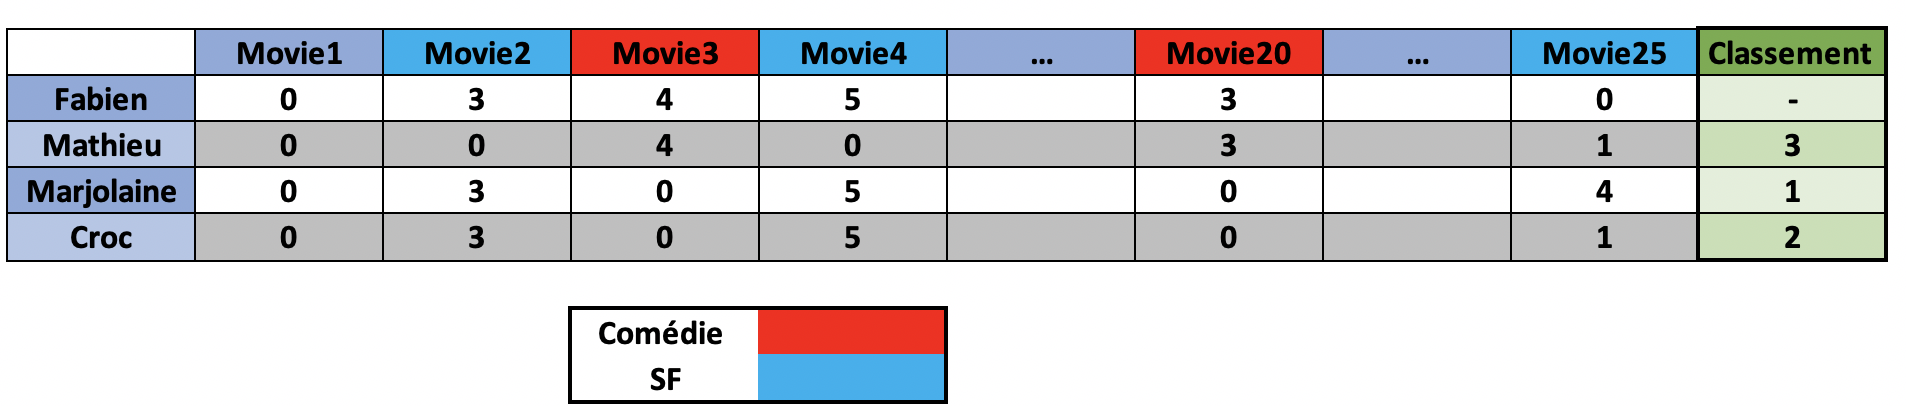
\includegraphics[width=95mm]{./src_img/apport_classement}
  \caption{Classement des voisins.}
  \label{fig:a-trois}
\end{figure}

\vspace{5mm}

\section{Prédiction}

Dans cette section, il faut prendre en compte plusieurs paramètres. Notamment si le genre du film sur lequel le système travaille à déjà au moins une évaluation par Fabien. On distingue deux cas : 

\vspace{5mm}

Le premier cas, si Fabien a déjà évalué au moins un film de Science-fiction, alors il faut calculer la différence entre la moyenne attribuée par Fabien au genre Science-fiction et la moyenne du voisin sélectionné pour ce même genre. Dans le cadre de mon développement, j’ai transformé la différence entre ces deux moyennes en un multiplicateur appelé « delta ». Le delta vaut exactement 1 si les deux utilisateurs ont une moyenne identique, le delta est négatif si Fabien note plus faiblement que le voisin sélectionné et inversement le delta est positif si Fabien note plus généreusement. Finalement, pour prédire la note du film, il faut multiplier la note donnée par le voisin par le delta. 

\vspace{5mm}

Le second cas, si Fabien n’a jamais attribué une note aux films de Science-fiction. Une moyenne donnée par Fabien pour le genre Science-fiction est impossible. J’ai choisi d’appliquer la même méthodologie que pour le premier cas mais sur les notes données de façon globale. Ainsi, je vais calculer la moyenne de toutes les notes données par Fabien et le voisin sélectionné. A partir des deux moyennes comme dans le premier cas, je vais créer un delta entre les deux moyennes. Finalement, pour prédire la note du film, il faut multiplier la note donnée par le voisin par le delta. 

\vspace{5mm}

Dans notre cas, Fabien a déjà attribué des notes à des films de Science-fiction avec une moyenne de 4 pour ce genre de film. Le profil voisin le plus proche est Marjolaine avec une moyenne de 4 attribuée sur les films de Science-fiction. Ici, le delta entre les deux moyennes à pour valeur 1 et Marjolaine a attribué la note de 4 au film "Jurassic World". Par conséquent, le système prédit que Fabien va attribuer une note de 4 pour le film "Jurassic World". 

\begin{verbatim}
Predict for Fabien
- - - - - - - - - - - - - - - - - - -
[0, 3, 4, 5, 0, 0, 0, 0, 0, 0, 0, 0, 0, 0, 0, 0, 0, 0, 0, 3, 0, 0, 0, 0, 4]
new rating : 4  
['Movie25', '2015', 'Jurassic World', 'Science-Fiction']
- - - - - - - - - - - - - - - - - - -
\end{verbatim}

\chapter{évalutation de mon apport}


\begin{center}
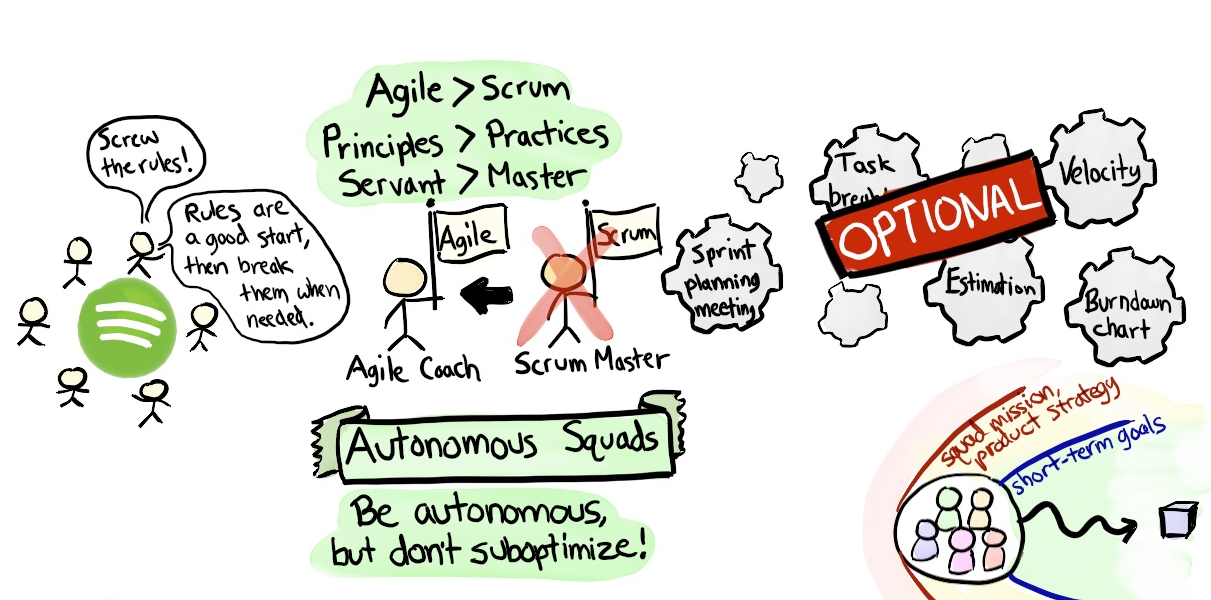
\includegraphics[width=95mm]{./src_img/agile_scrum}
\end{center}

\begin{figure}[htp]
  \centering
  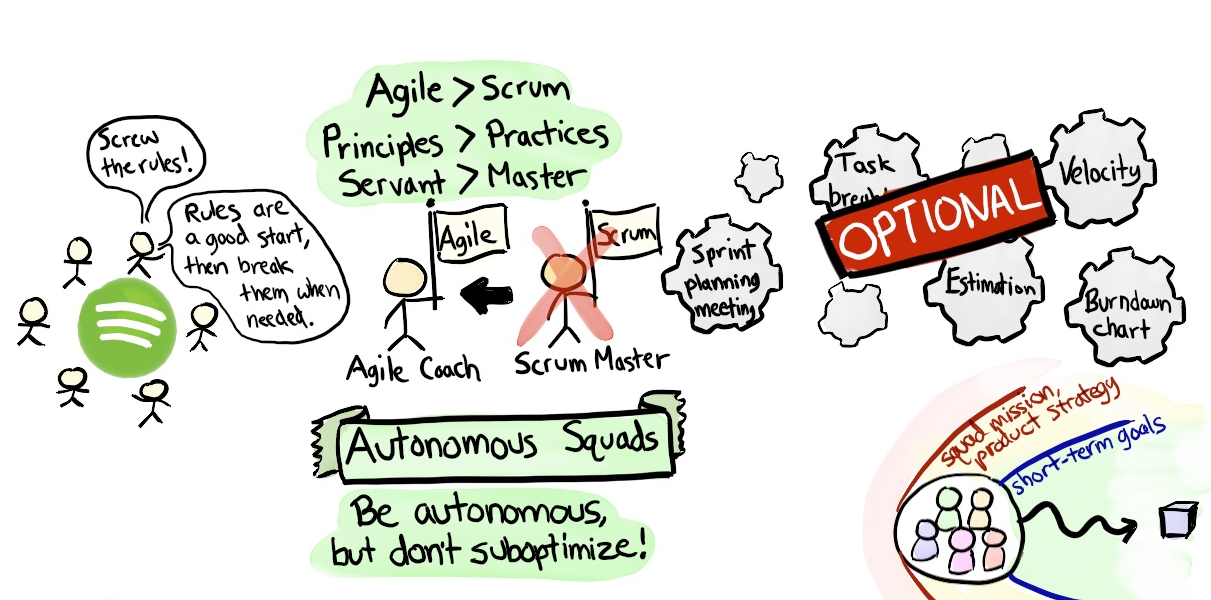
\includegraphics[width=95mm]{./src_img/agile_scrum}
  \caption{Organigramme du LRI.}
  \label{fig:une-autre-image}
\end{figure}




Lorem ipsum dolor sit amet, consectetur adipiscing elit. Maecenas ultricies, felis iaculis interdum ultrices, sem elit mollis diam, in porta velit magna vitae elit. Fusce vestibulum mollis sapien dapibus rhoncus. Ut ut auctor urna. Vivamus viverra lacinia est, ut facilisis enim bibendum in. Vivamus mollis mollis metus. Maecenas sagittis ipsum id dignissim molestie. Praesent et dignissim quam. Curabitur tristique mi ut eros elementum, at gravida magna dignissim. Aliquam imperdiet sollicitudin arcu et viverra. Phasellus eu cursus nibh.

Etiam ut urna viverra, vestibulum ipsum sed, auctor orci. Cras id cursus quam, sit amet feugiat nunc. Ut sed nibh eget massa varius ornare et viverra sem. Nulla facilisi. Duis luctus erat mauris, vitae lacinia sapien imperdiet sit amet. Duis tincidunt sem a tristique efficitur. Praesent eget augue in metus maximus gravida. Maecenas in fermentum purus. Praesent at leo at nunc eleifend hendrerit. Aenean tempus, mi at lacinia aliquet, metus velit faucibus mi, vitae maximus tellus nulla molestie neque. Proin tristique scelerisque enim sit amet fringilla. Sed porta metus a tristique semper.

In molestie, tortor vel sodales ornare, massa ligula volutpat dolor, ac ullamcorper lorem dui non dui. Pellentesque sollicitudin elit vitae sem tristique aliquet. Nullam fringilla mi eu dui rhoncus malesuada. Pellentesque faucibus, leo eget euismod consequat, nibh mi euismod mauris, quis porta mi arcu non enim. Integer nec arcu faucibus, varius enim at, condimentum nisl. Suspendisse nec feugiat nibh. Nullam aliquet justo ut mi imperdiet, vel ultrices arcu rhoncus. Donec eu sem sit amet mauris sodales semper. Cras pharetra malesuada turpis. Pellentesque hendrerit pellentesque pellentesque. Aenean varius, orci vehicula rhoncus luctus, lectus mi tincidunt massa, vel viverra leo ante efficitur risus. Proin in feugiat nunc.

Maecenas facilisis risus ut neque maximus, at sollicitudin ante cursus. Integer convallis eleifend purus, at maximus massa maximus sed. Praesent fermentum aliquet viverra. Mauris tristique suscipit lobortis. Aenean ornare nibh hendrerit metus sodales, at faucibus nunc auctor. Integer imperdiet fermentum congue. Sed eu dui vel elit iaculis posuere vitae et nulla. Vivamus laoreet ut erat non tempus. Ut vitae enim nisi. Donec finibus cursus mi ut porttitor.

Morbi sollicitudin sem at venenatis placerat. Integer quis diam tempor, vulputate diam nec, aliquam mi. Nulla sit amet arcu sollicitudin, rhoncus metus vel, facilisis diam. Duis ut pulvinar sapien. Lorem ipsum dolor sit amet, consectetur adipiscing elit. Maecenas viverra velit nec laoreet fermentum. Sed vestibulum magna ac molestie tempus. 

\chapter{Évolutions possibles}



Dans ce chapitre, je vais décrire les évolutions possibles concernant le  « Netflix Prize »  puis celles de Netflix et enfin celles de mon apport.

\vspace{5mm}

Concernant le « Netfliz Prize », l’équipe BellKor’s Pragmatic Chaos est la première équipe à avoir remporté le Netlflix Prize challenge avec un RMSE meilleur que l’algorithme Cinematch.  Ce concours a permis une avancée considérable pour des systèmes de recommandation mettant en avant la puissance de la factorisation matricielle pour le filtrage collaboratif mais aussi l’émergence de nouveaux algorithmes pour le machine learning. Netflix a autorisé l’utilisation des données mise à disposition pour la recherche, ce qui permet encore actuellement des avancées et des recherches sur l’approche des systèmes de recommandation et leur évolutivité. De nombreuses personnes déposent leurs solutions sur des outils de partages collaboratifs comme GitHub par exemple. Le Netflix Prize ne permettra plus de générer autant d’enthousiasme de la part des chercheurs et passionnés qu’entre 2006 à 2009. Cependant, il n’est pas impossible qu’un nouvel algorithme issu de ce challenge bouscule le monde de la recommandation. 


\vspace{5mm}


Au sujet de Netflix, avec l’arrivée de nouveaux concurrents, la plateforme doit perpétuellement se renouveler. Une grande partie de son budget est utilisé pour l’acquisition de droit sur des contenus, comme pour la série "Friend" mais aussi pour la création de contenus originaux. La création de contenus originaux est un choix logique et raisonné. En effet, de nombreux acteurs prennent leur independance comme Disney, ce qui induit une perte des droits pour Netflix de beaucoup de licence forte comme l’ensemble des films PIXAR. A court terme, il est logique d’imaginer que Netflix va utiliser ses points forts pour garder ses utilisateurs et en acquérir de nouveaux. Comme démontré tout au long de ce mémoire, la grande force de Netflix est représentée par son système de recommandation à partir duquel 80\% du contenu consommé provient. Il est logique de penser que Netflix va utiliser son système de recommandation pour mettre en avant des contenus exclusifs à la plateforme. Logiquement, les futures évolutions de Netflix côté software se baseront sur l’interface mais principalement sur l’amélioration continue de leur algorithme de recommandation permettant ainsi de diminuer petit à petit la marge d’erreur du système de recommandation bien quelle soit aujourd’hui déjà négligeable. 


\vspace{5mm}

Pour finir, concernant mon apport, il existe plusieurs axes d’améliorations. Premièrement, une amélioration de la fiabilité et la qualité de mes algorithmes permettrait de pousser la prédiction plus loin. Une prédiction plus fiable permet de produire une note pratiquement aussi fiable que celle donné explicitement par l’utilisateur et donc d’être utilisée pour prédire d’autres films. Par exemple, si un utilisateur n’a jamais regardé de Comédie et qu'une première prédiction a mis en évidence une prédiction fiable pour un film Comique, une seconde étape pourrait être l’exploitation de cette note pour recommander d’autres films dans le genre Comédie. 

\vspace{5mm}

Secondement, j’ai essayé de démontrer que prendre en compte une seconde donnée tel que le genre du film permettait d’apporter une information pertinente et ce malgré la complexité supplémentaire. Je suis convaincu que l’utilisation de sous-genre comme les Comédies Romantiques permettrait d’augmenter la pertinence de la recommandation. L’utilisation de l’année du film serait sûrement une autre voie à explorer, permettant ainsi de déterminer si l’utilisateur préfère les films anciens ou plus récents. 

\vspace{5mm} 

Rétrospectivement en analysant mon travail, j’ai appliqué deux fois l’algorithme des plus proches voisins. Il serait sûrement plus pertinent d’utiliser plusieurs algorithmes sur plusieurs dimensions comme l’équipe gagnante du « Netflix Prize ». Je pense que l’agrégat des recommandations issu de plusieurs algorithmes offre une force supplémentaire afin d’obtenir une recommandation plus qualitative et plus pertinente. 



\chapter*{Conclusion}
\addcontentsline{toc}{chapter}{Conclusion}
\markboth{Conclusion}{Conclusion}
\label{sec:conclusion}




Lorem ipsum dolor sit amet, consectetur adipiscing elit. Maecenas ultricies, felis iaculis interdum ultrices, sem elit mollis diam, in porta velit magna vitae elit. Fusce vestibulum mollis sapien dapibus rhoncus. Ut ut auctor urna. Vivamus viverra lacinia est, ut facilisis enim bibendum in. Vivamus mollis mollis metus. Maecenas sagittis ipsum id dignissim molestie. Praesent et dignissim quam. Curabitur tristique mi ut eros elementum, at gravida magna dignissim. Aliquam imperdiet sollicitudin arcu et viverra. Phasellus eu cursus nibh.

Etiam ut urna viverra, vestibulum ipsum sed, auctor orci. Cras id cursus quam, sit amet feugiat nunc. Ut sed nibh eget massa varius ornare et viverra sem. Nulla facilisi. Duis luctus erat mauris, vitae lacinia sapien imperdiet sit amet. Duis tincidunt sem a tristique efficitur. Praesent eget augue in metus maximus gravida. Maecenas in fermentum purus. Praesent at leo at nunc eleifend hendrerit. Aenean tempus, mi at lacinia aliquet, metus velit faucibus mi, vitae maximus tellus nulla molestie neque. Proin tristique scelerisque enim sit amet fringilla. Sed porta metus a tristique semper.

In molestie, tortor vel sodales ornare, massa ligula volutpat dolor, ac ullamcorper lorem dui non dui. Pellentesque sollicitudin elit vitae sem tristique aliquet. Nullam fringilla mi eu dui rhoncus malesuada. Pellentesque faucibus, leo eget euismod consequat, nibh mi euismod mauris, quis porta mi arcu non enim. Integer nec arcu faucibus, varius enim at, condimentum nisl. Suspendisse nec feugiat nibh. Nullam aliquet justo ut mi imperdiet, vel ultrices arcu rhoncus. Donec eu sem sit amet mauris sodales semper. Cras pharetra malesuada turpis. Pellentesque hendrerit pellentesque pellentesque. Aenean varius, orci vehicula rhoncus luctus, lectus mi tincidunt massa, vel viverra leo ante efficitur risus. Proin in feugiat nunc.

Maecenas facilisis risus ut neque maximus, at sollicitudin ante cursus. Integer convallis eleifend purus, at maximus massa maximus sed. Praesent fermentum aliquet viverra. Mauris tristique suscipit lobortis. Aenean ornare nibh hendrerit metus sodales, at faucibus nunc auctor. Integer imperdiet fermentum congue. Sed eu dui vel elit iaculis posuere vitae et nulla. Vivamus laoreet ut erat non tempus. Ut vitae enim nisi. Donec finibus cursus mi ut porttitor.

Morbi sollicitudin sem at venenatis placerat. Integer quis diam tempor, vulputate diam nec, aliquam mi. Nulla sit amet arcu sollicitudin, rhoncus metus vel, facilisis diam. Duis ut pulvinar sapien. Lorem ipsum dolor sit amet, consectetur adipiscing elit. Maecenas viverra velit nec laoreet fermentum. Sed vestibulum magna ac molestie tempus. 



\newpage
%\nocite{SpaceXFirstISS, IFPI2011Report, SpotifyBloomberg, SpotifyNewYorker}
\printbibliography

\newpage
\listoffigures

\newpage
\thispagestyle{empty}
\vspace*{\fill}
\begin{center}
  Université Paris-Nanterre\\
  200 Avenue de la République\\
  92000 Nanterre
\end{center}
\vspace*{\fill}

\end{document}